\chapter{The Value Behind Traffic}

% \begin{tabular}{c}
    \textbf{The Value Behind Traffic: How Patient Discretion and Information Coarseness Altered Healthcare Traffic in the Wake of COVID-19.}
    This Chapter is co-authored with Dr. Bradley Staats.
% \end{tabular}

% \begin{center} \rule{6in}{0.01in} \end{center}
% \noindent 
%  \textbf{Chapter Abstract:} \\
%  \textbf{Background:} Traffic represents a key operational input, especially in healthcare. Many aspects of medicine cannot happen from a distance, and serious consequences follow delayed or omitted care. And yet with the emergence of Covid-19 in March of 2020, traffic to many clinics vanished overnight. \\
%  \textbf{Aim:} Using empirical methods, we aim to explore how the value of the service consumed impacts healthcare clinic traffic. We also examine how traffic changed with coarse and precise signals of the pandemic environment. \\
%  \textbf{Methods:} Our study combines observations from healthcare clinics across 15 US states, anonymized cellphone mobility data, Covid-19 severity measures, and state-wide stay-at-home orders. A Lasso-based procedure from machine learning non-arbitrarily selects instruments and generates exogenous county-level measures of individual mobility. \\
%  \textbf{Results:} Clinic traffic returns with rising personal mobility, but the size of returns vary by the type of service: A 1\% increase in mobility yields a 2\% return to vaccination traffic but only a 0.5\% return to non-vaccination traffic. And the response to signals depends on signal severity and treatment sought: While precise signals affect non-vaccination traffic more than coarse signals, vaccination traffic seems immune to such factors. \\
%  \textbf{Conclusions:} During the pandemic, preferences emerged and patients exercised discretion in ways many feared. Encouragingly, we find patients prioritized important services and shouldered some of the burden of their own wellness. By studying such decisions, we identify and characterize powerful predictors of healthcare clinic traffic, and we encourage researchers to explore the role of patient discretion in the co-production of wellness. 
% \begin{center} \rule{6in}{0.01in} \end{center}
%  \noindent\keywords{Traffic; Vaccinations; Healthcare Operations; Empirical Operations; Machine Learning }

\section{Introduction}
 Customer traffic drives many aspects of company operations \citep{Gallino2014}. \cite{Perdikaki2012} argue retailer profitability directly depends on the ability to understand traffic, for several reasons. First, traffic informs labor planning \citep{Mani2015,Chuang2015,Perdikaki2017,Netessine2010}. Second, variation in traffic can highlight operational problems in other areas \citep{Lee2017}. And finally, understanding traffic patterns enables better traffic prediction \citep{Yung2020,Kamalahmadi2021,Abrishami2018}. Traffic represents a key operational input -- especially in healthcare. Even with growing acceptance of telemedicine \citep{WSJ_21_telemed,Friedman2021}, limits remain: a physician cannot perform a physical or administer vaccines without seeing patients in-person. For now, many aspects of healthcare cannot happen when separated \citep{Romanick-Schmiedl2020} and serious consequences follow delayed or omitted care \citep{Findling2020,CDC_ExcessDeath}. Operational success depends on understanding traffic -- and the events surrounding March 2020 drive this point home in healthcare.
 % Operational success depends on understanding traffic, and the events of, and subsequent to, March 2020 drive this point home with clarity in healthcare
 
 With the emergence of the SARS-CoV-2 virus and the associated disease (Covid-19), traffic to many clinics vanished overnight. Some preventive care measures dropped by more than 80\% \citep{Cantor2020}. The declines were so precipitous and so concerning, a campaign in July 2020 advised: “Stay 6 feet away from others, stay close with your doctor" \citep{StopMedicalDistancing.org}. Such drops possess grave implications for patient \citep{WSJ_skipDoc} and physician \citep{WSJ2020_job_losses} welfare, and so we ask: “What factors drove healthcare clinic traffic during the Covid-19 pandemic?" Our work empowers clinics to better meet patient needs \citep[as in][]{Musalem2020} and accurately predict traffic moving forward. 
%  perhaps as much as 50\% of the US population delayed some type of care in 2020 \citep{Findling2020}.

 To date, as evidenced by the plethora of studies listed in \cite{Gupta2020}, the state-wide “stay-at-home" or “shelter-in-place" orders remain the literature's primary concern. But stay-at-home orders cannot fully explain the drop in clinic traffic. Many states issued orders, but most clinics remained open through exemptions for “essential services." Moreover, individual decisions and personal preferences appear to drive willingness to engage with in-person activities more than the state-wide orders \citep{Goolsbee2020_key}. Figure \ref{fig:t2_mot_fig} affirms this insight using observations from our study: \textit{Personal mobility} (i.e., Trips per Person), which captures a willingness to travel, drops even before stay-at-home orders go into effect. And so our paradigm evolves: To improve patient health, see most patients in-person. To see them in-person, you have to be open. But just being open cannot suffice: Patients must also decide that they want to be seen.
 % To address certain aspects of patient health, you must see patients in-person. To see patients in-person, you have to be open. But just being open cannot suffice: Patients must also decide that they want to be seen.
 
 \begin{figure}[!b]
    \centering
    \caption{Trips per Person, or personal mobility, drops before shutdown orders go into effect. The drop also coincides with an increase in search engine interest in Covid-19.}
    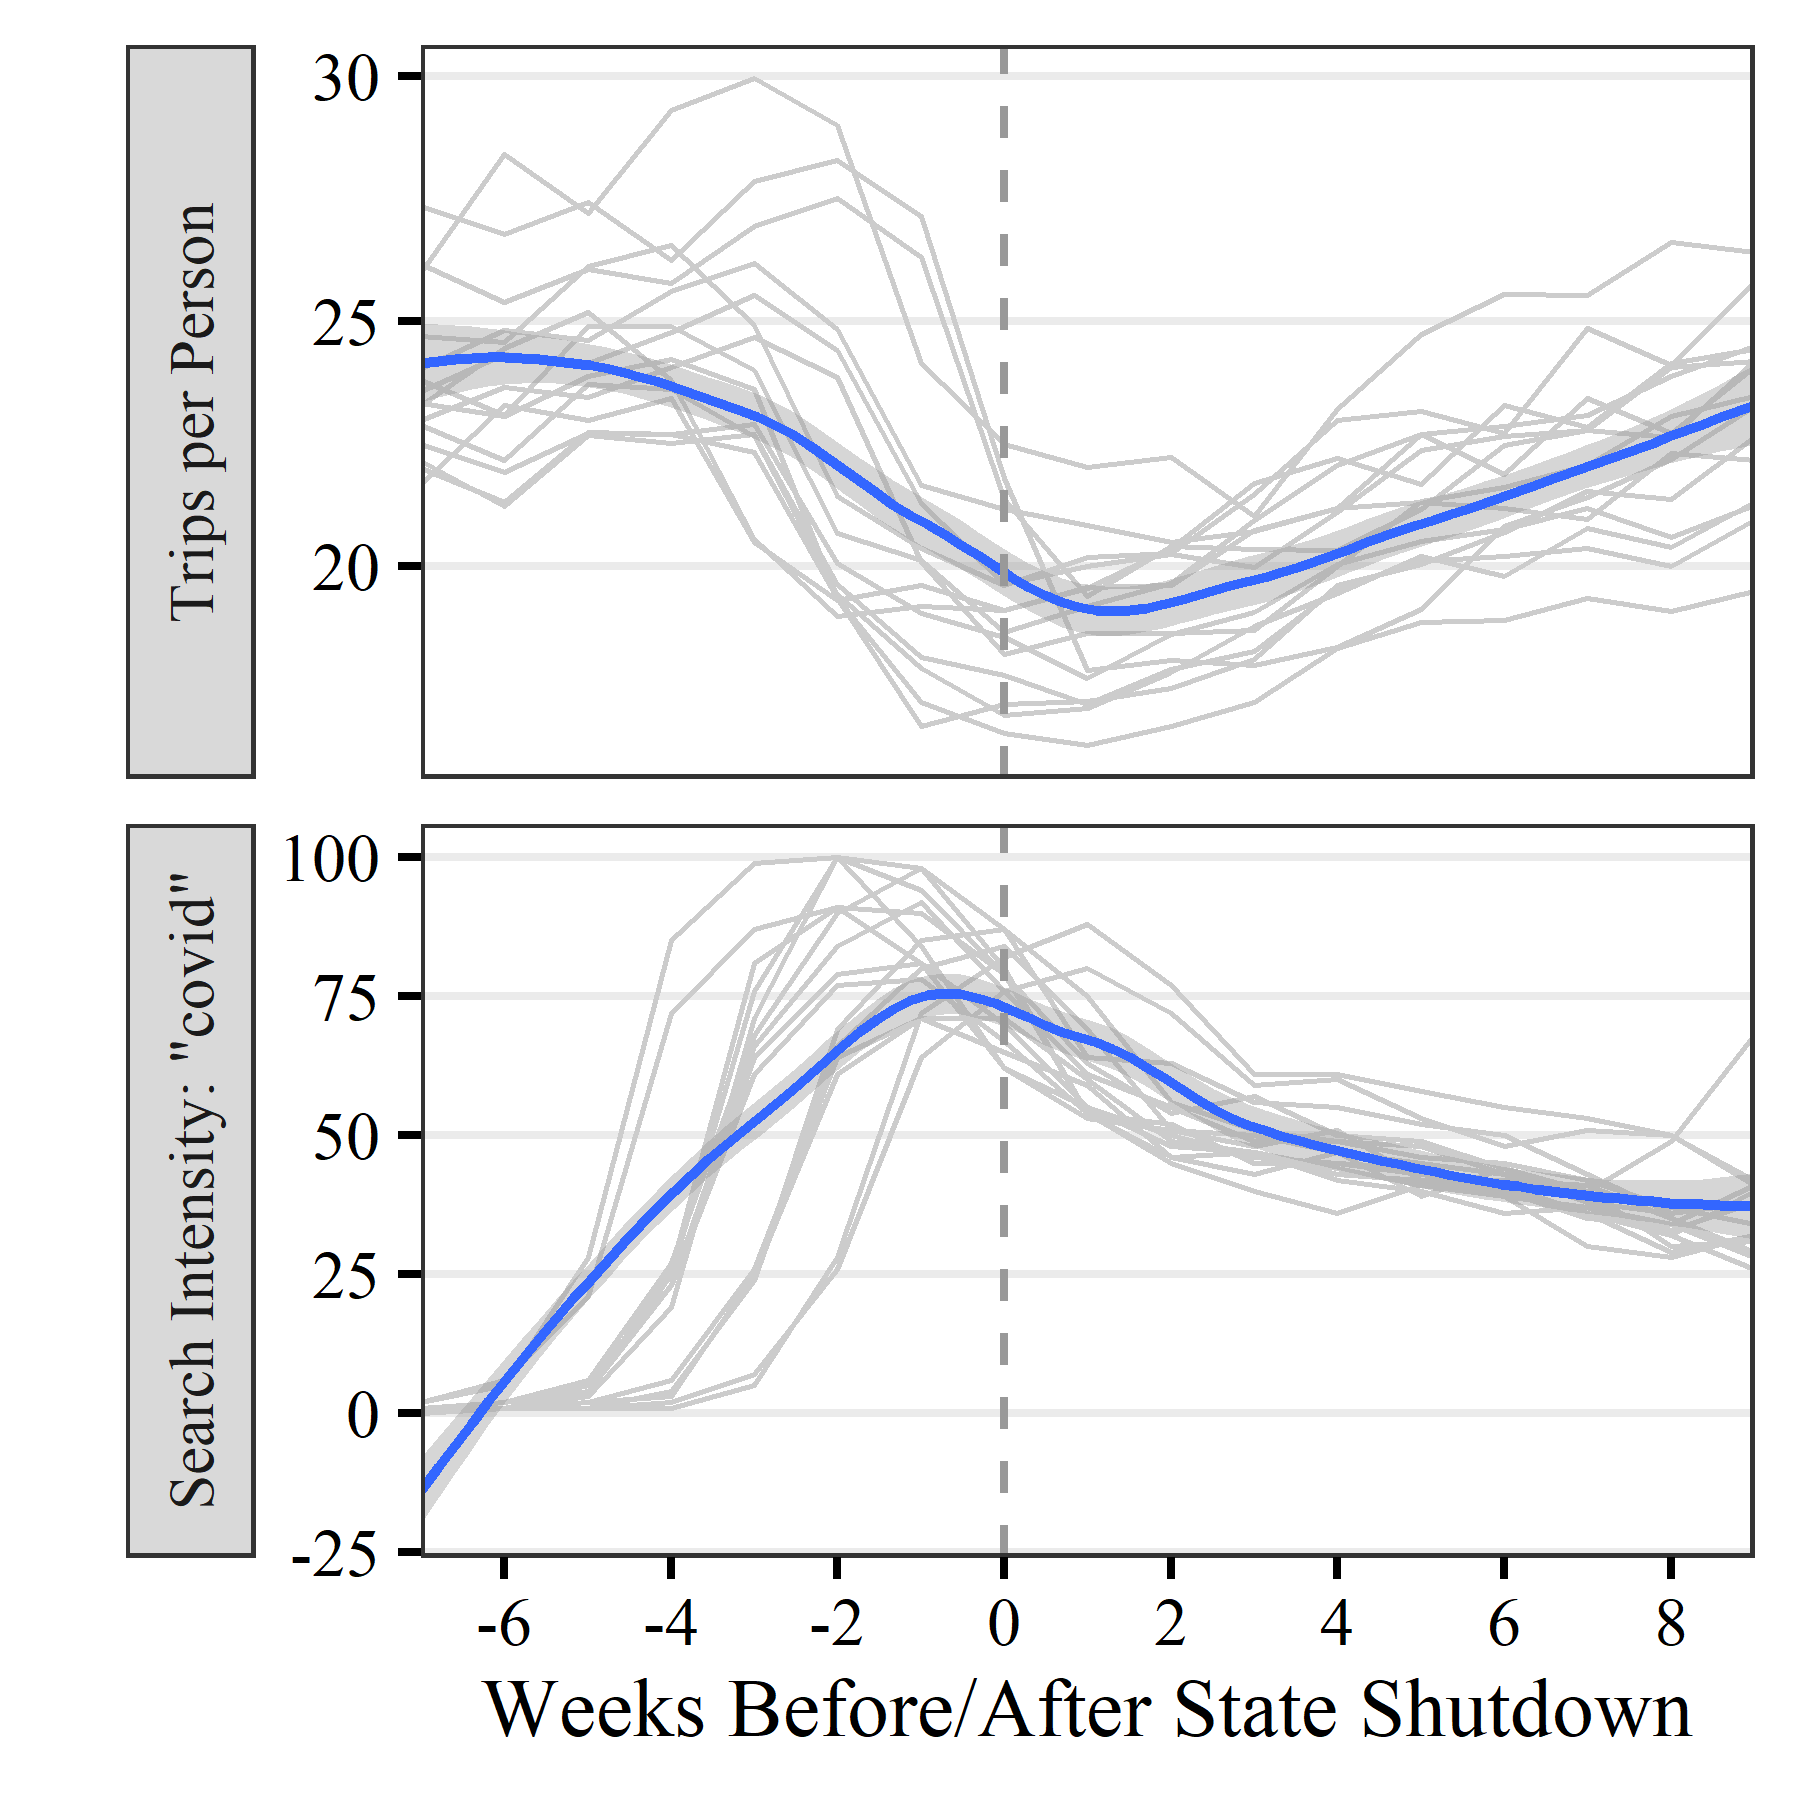
\includegraphics[scale=1]{Figures/VC2/MotFig-Take2.png}     
    \label{fig:t2_mot_fig}
    \floatfoot{\textbf{Figure Note:} The figure plots mobility and search data for 15 US states relative to the stay-at-home order for each state. The 15 states represent the states for which we also have clinic traffic observations (Section \ref{data}). The blue line depicts a “Loess" conditional smoothing function applied to the raw data. The graph illustrates “Trips per Person" as recorded by the \cite{MTI2020}. “Search Intensity" represents user searches for the word “covid" from \cite{Google2021_covid}, where intensity varies from very few to many searches on a scale from 0 to 100. }
 \end{figure}  
 
 What then influences the decision to be seen? Executive orders might influence some behavior, but patient discretion and personal preferences likely dictate mobility just as much if not more. In contrast to such orders, Figure \ref{fig:t2_mot_fig} shows a drop in mobility coincides with an increase in Google search intensity. Perhaps mobility drops with greater fear of Covid \citep{Alfaro2020}, but then what drives such fear? Signals of environmental safety could incite fear, either as a coarse mandate (e.g., “Stay home: it is not safe to go out") or a precise nudge (e.g., “10\% of people in your area are sick"). But for every push, see a pull: Fear compels someone to stay home, and \textit{value} invites someone to go out. Since there is discretion in movement -- where an individual can choose between staying or going -- we must then consider the value generated by such movement.
 
 In the end, because high-value trips might lead patients to travel more, traffic predictions need to account for movement value. If mobility drops but remains non-zero (see Figure \ref{fig:t2_mot_fig}), then trips that remain must generate greater value than trips that fade. Hence, we ask: “During the pandemic, how does the value of the service consumed impact healthcare clinic traffic?" We operationalize the question by comparing general trips to a clinic (less valuable) to trips which specifically include vaccination (more valuable). Clinic “traffic" nests both, and both serve important roles in patient health. But delaying or omitting vaccinations poses immediate risks to the patient and the community \citep{Salmon2015,Brewer2017}; the flu vaccine alone averts tens of thousands of hospitalizations each year \citep{CDC2020_flu}. And so we examine the pull of different services and discuss the implications for clinic traffic predictions. 
 % In studying traffic, it is important to account for movement value as  
 % Cite Brewer? Phadke?

 Our approach also models how information signals shape the decision to travel. A high-value goal may incentivize traffic, but environmental signals should also influence the calculation of value. In particular, we consider signal \textit{coarseness} \citep{Morris2007}: Executive, state-wide stay-at-home orders represent coarse signals of environmental safety while local, publicly available Covid metrics (e.g., case counts) represent precise signals. To answer our research questions, our study combines observations from: Healthcare clinics across 15 US states; anonymized county-level cell phone mobility observations; county-level Covid-19 measures; and public information on state-wide stay-at-home orders. During our study period, three factors interact to shape healthcare clinic traffic: (i) individual mobility preferences, (ii) the value of the care sought, and (iii) the perception of disease severity.
 % We also explore whether the severity of the precise signals matters by comparing changes in the effect of mobility with signals of lower severity (Covid case counts) and signals of higher severity (Covid death rates).
 
 Based on our empirical analysis, we find the following. \textbf{First}, clinic traffic returns with rising personal mobility. The size of such returns, however, vary significantly: A 1\% increase in mobility yields a large return to vaccination traffic (+2.169\%) but a fractional return to non-vaccination traffic (+0.56\%). More mobility means more traffic, depending on the type of care and value provided, one contribution of our study. \textbf{Second}, precise signals dominate coarse signals in affecting non-vaccination traffic. Precise signals also attenuate the effect of mobility on such traffic, especially when signaling even greater hazard (e.g., rising Covid death rates). In choosing information coarseness, trade-offs abound in the literature. We contribute to the debate by comparing one coarse signal, which has no impact, to precise signals which alter both mobility decisions and clinic outcomes. \textbf{Finally}, aside from personal mobility, no other factors have any detectable impact on vaccination traffic. Priorities emerged as states started reopening and people decided to leave home, revealing people may consider vaccinations more important than other elements of primary care. By studying the effect of such decisions, we identify and characterize powerful predictors of healthcare clinic traffic.

 In executing our study, we also add to emerging literature exploring effects of the Covid-19 pandemic. As surveyed in \cite{Gupta2020a}, most studies focus on the implications of stay-at-home orders; many examples exist in economics \citep[e.g.,][]{Goolsbee2020_key,Goolsbee2020_unpub,Alfaro2020,Cantor2020,Alfaro2021,Ziedan2020,Farboodi2020,Zhang2020}, though we know of only one published example in operations \citep{Wang2021}. As discussed in \cite{Wang2021}, such studies generally focus on mobility as the outcome of interest (p. 4). In contrast, our study considers mobility the aggregated decisions of individuals which then act as an input and predictor for our outcome, clinic traffic. To the best of our knowledge, no other studies have used personal mobility to predict changes in traffic during the pandemic. We also contribute by leveraging developments in machine learning to enhance our identification strategy.
 
 In Section \ref{VC2_HD}, we position our study in the broader literature which we use to develop and motivate our hypotheses. Section \ref{VC2_Emp} describes our data and our empirical strategy. Section \ref{VC2_Results} presents our results and a post-hoc analysis. Section \ref{VC2_Conc} concludes.
  

\section{Hypothesis Development} \label{VC2_HD}
\subsection{Mobilizing Differently: The Effect of Value}
 In operations, traffic represents a critical input for many system-level outcomes \citep[e.g.,][]{Perdikaki2012}. Without an adequate understanding of traffic, other operational efforts may yield no benefit, including efforts like inventory management or queue design. For example, traffic informs labor planning \citep[e.g.,][]{Chuang2015} and inadequate labor planning can lead to poor service and employee attrition \citep{Ton2008}. \cite{Lee2017} illustrate a retail situation where high traffic and insufficient staffing lead to “phantom stockouts" because inventory is shelved incorrectly. And low traffic to clinics \cite[such as documented by][]{Mehrotra2020,Mehrotra2021} erodes clinic revenue and limits the ability of providers to monitor chronic conditions. In sum: Unanticipated traffic in either direction complicates operational planning.
 
 Even so, individual willingness (or reluctance) to travel precedes clinic traffic; we refer to such willingness as “personal mobility." While some studies explore how mobility affects other factors \citep[e.g., the spread of infection in][]{Dave2020}, the emerging literature in economics mostly focuses on how the stay-at-home orders orders affect mobility \citep[review in][]{Gupta2020}. And yet \cite{Goolsbee2020_key} argue individual reluctance to venture out dominates the effect of the stay-at-home orders. Similar implications emerge for preventative, elective, and outpatient traffic \citep{Ziedan2020,Cantor2020}, but such studies lack a coherent reason for why patients delayed some elements of care but not others \citep{Czeisler2020}. Factors beyond just state-wide stay-at-home orders might explain variance in clinic traffic better.
%  Cite Dave2021?
 
 We propose the value of the care informs personal mobility which then drives clinic traffic. One case in point: Early in the pandemic the American Medical Association issued guidelines to help private practices “triage" different types of care \citep{AmericanMedicalAssociation2020}. The guidelines included assessing patient risk and treatment urgency, two inputs to the value of care. To operationalize value, we classify non-vaccination traffic as less valuable and vaccination traffic as more valuable; we then study how personal mobility decisions affect the two types of traffic. Patients delayed or omitted less valuable care at record levels during 2020 \citep{WSJ_pcp,WSJ_skipDoc}, while the medical community claims “... vaccination is one of public health’s greatest achievements" \citep[p. 190]{Brewer2017}. In fact, industries such as healthcare and education commonly require vaccination records for employees and patrons \citep{CDC_stateVaccReq}. Given such differences and conditional on a willingness to leave home, we propose more valuable care will return faster than less valuable care with increasing mobility.
%  even emergency departments saw drastic reductions in care \citep{Hartnett2020}.

 \medskip \noindent
 \begin{tabularx}{\linewidth}{ r X }
    \textbf{Hypothesis 1:} & \textit{An increase in personal mobility will correspond to \underline{greater} returns to more valuable care (vaccination traffic) than to less valuable care (non-vaccination traffic).} [H1]
 \end{tabularx}   %\medskip

\subsection{Mobilizing Safely: The Effect of Signaling}
 Next, we explore the effect of different types of public information on clinic traffic. In philosophy and economics, studying the “social value of public information" or signals extend back decades \citep[p. 1]{Morris2002}. \cite{Lewis1969} argues that signaling conventions yield what \cite{Grice1957} calls “meaning," where common knowledge of a signal's intention represents a key element of conventions. Said differently: Common knowledge begets conventions. Conventions reveal the intentions of a signaler and facilitate shared understanding. And “[successful] communication rests on shared understanding" \citep[p. 594]{Morris2007}.
 
 Pursuing shared understanding, however, might compromise signal precision through an increase in information \textit{coarseness} \citep{Morris2007}. For example, assigning a coarse grade of “Pass" instead of a precise “73/100" might yield broader comprehension \citep{Harbaugh2018}. In such a decision, trade-offs abound: Coarse information is easier to process \citep{Harbaugh2018} and increases the likelihood of “shared understanding," but “unsophistication" and imprecision can also lead to welfare loss \citep{Morris2007}. On the other hand, less coarse information might be easier to use \citep{Morris2007,Chahrour2017}, though such an approach risks information overload \citep{Eppler2010} and complicates coordination \citep{Morris2002}. Experienced signalers tailor information coarseness to balance the trade-offs.
 
 During the pandemic, policy makers released information of varying coarseness to signal how safe it was to move about. In our study, state-wide stay-at-home orders represent coarse signals. Such orders, typified in the executive orders issued by state governors, issued general guidance and included mandates which closed down sections of the economy without providing specific information on the current disease state. In contrast: Local, publicly available Covid metrics, such as those available through the \cite{NYTimes2021} or from \cite{JHU2021}, represent precise signals. In our study, we compare two different precise signals which communicate low-severity (new Covid cases) and high-severity metrics (Covid death rate). We then explore how coarse and precise pandemic signals affected clinic traffic.
 
 What might we expect to find? Despite their prevalence, the full effect of stay-at-home orders on clinic traffic remains murky. Yes, traffic dropped -- but such orders can only explain a portion of the declines \citep{Cantor2020,Ziedan2020}. Perhaps the orders characterized an environment which conflicted with individual experience, and people tend to ignore or override new information which conflicts with experience \citep{Staats2018,Kesavan2020}. Or perhaps precise signals affect clinic traffic more than the coarse stay-at-home orders, since (i) “individual choices were far more important [than the orders]" \citep[p. 1]{Goolsbee2020_key}, and (ii) the choices “seem tied to fears of infection" \citep[p. 1]{Goolsbee2020_key}, where (iii) “fear has a robust negative association with mobility that extends beyond any government response" \citep[p. 15]{Alfaro2020}. In fact, \cite{Goolsbee2020_key} find one type of precise signal (Covid deaths) reduces retail traffic even after controlling for other factors. Thus, we hypothesize precise signals will serve as a stronger predictor of clinic traffic than coarse signals, though we allow the effect to vary by the inherent value of each traffic type, in line with Hypothesis 1. 
%  , particularly since people ignore good advice more often then they should \citep{Bonaccio2006}.
 
 \medskip \noindent
 \begin{tabularx}{\linewidth}{ r X }
    \textbf{Hypothesis 2a:} & \textit{Precise, local signals of environmental safety (new Covid cases and Covid death rate) \underline{more negatively} impact \textbf{non-vaccination traffic} than coarse, state-wide stay-at-home orders.} [H2a]  \\
    \textbf{Hypothesis 2b:} & \textit{Precise, local signals of environmental safety (new Covid cases and Covid death rate) \underline{more negatively} impact \textbf{vaccination traffic} than coarse, state-wide stay-at-home orders.} [H2b] 
 \end{tabularx}   % \medskip
 
 
\section{Empirical Setup} \label{VC2_Emp}
\subsection{Data Description} \label{data}
 To address our research questions empirically, we partnered with VaxCare, a vaccine management company headquartered in Orlando, FL. VaxCare partners with health care clinics to manage vaccination logistics, including ordering vaccines from the manufacturer, managing clinic inventory, and billing respective payers. VaxCare partner clinics vary in size and specialty, from smaller, regional pediatric offices to larger networks of clinics. Although pediatric vaccines are frequently thought of first, adult vaccines, such as shots for shingles or pneumonia, are also critical life-saving tools and represent about 30\% of our sample. VaxCare has provided observations from their distributed clinic network which contains hundreds of clinics in 15 different US states: Alabama, Colorado, Florida, Georgia, Illinois, Indiana, Kansas, Kentucky, Missouri, New York, Ohio, Oklahoma, Pennsylvania, South Carolina, and Texas. Although VaxCare’s technology infrastructure tracks clinic vaccinations for all partners, a subset of partners maintain a closer integration with the VaxCare network. For such clinics, VaxCare also observes clinic traffic. Please see Appendix \ref{app_clinicSelection} for our clinic inclusion criteria.
 
 We merge the clinic observations with 2020 county-level information from the University of Maryland’s Covid-19 Impact Analysis Platform \citep{MTI2020}. The dataset includes personal mobility measures (such as miles traveled and the number of trips taken) collected from anonymized cell phone data by companies like Apple, Google, and SafeGraph; because such data enables valuable location-based services, very few smartphone users opt-out of collection \citep{Anderson2016}. The platform also integrates Covid-19 case metrics collected from \cite{JHU2021}. To such measures the platform adds other publicly available measures, such as hospital utilization, local unemployment rate, and county demographics (gender, population, median income, etc.).  also use such data. We refer interested readers to (a) \cite{Zhang2020} for a complete discussion of the platform, and to (b) \cite{Wang2021} as a published example of a study using similar data. 
 
 To our observations, we added publicly available knowledge of state-wide stay-at-home orders, frequently referred to as “shelter-in-place" or “stay-at-home" orders. \cite{Goolsbee2020_unpub} collected and made the information publicly available, and we verified the dates via other public sources, such as state executive orders as catalogued by \cite{Ballotpedia2020}. 
 
 Table \ref{tab:summary_stats} reports weekly summary statistics for key variables before, during, and after the stay-at-home orders. For our regression models, in order to focus our study on the early effects of the pandemic surrounding the orders, we split our observations into two separate samples. The first sample includes observations from January through February, 2020. The sample provides a pre-pandemic baseline for several of our metrics. The second sample includes observations from March 1 through 60-days following the lifting of the stay-at-home orders, which vary by state for each clinic. We evaluate our hypotheses during the second sample period, using changes relative to the pre-pandemic baseline, similar to \cite{Goolsbee2020_key}.

 \begin{table}[htbp]
 \resizebox{.8\textwidth}{!}{ 
 \begin{threeparttable}[t]
  \centering
  \caption{Weekly Averages (Standard Deviations) by State-level Operating Condition ($n = 172$ clinics)}
    \begin{tabular}{rccc}
          & \textbf{Before} & \textbf{During} & \textbf{After} \\
          & \textbf{Shutdown} & \textbf{Shutdown} & \textbf{Shutdown} \\
          &       &       &  \\
    Total Clinic Traffic & 277.02 & 186.04 & 222.00 \\
          & (5.12) & (5.57) & (5.37) \\
    Non-Vaccination Traffic & 264.64 & 178.07 & 209.30 \\
          & (4.99) & (5.34) & (5.17) \\
    Vaccination Traffic (no. shots) & 22.81 & 17.05 & 23.58 \\
          & (0.77) & (1.32) & (1.11) \\
    Trips (per person) & 24.17 & 19.35 & 21.71 \\
          & (0.1) & (0.11) & (0.08) \\
    New Covid Cases (per 1000 people) & 0.34  & 0.62  & 0.49 \\
          & (0.02) & (0.05) & (0.02) \\
    Covid Death Rate & 1.01\% & 17.04\% & 11.54\% \\
          & (0.05\%) & (0.21\%) & (0.09\%) \\
    New Unemployment Claims (per 1000 people) & 15.79 & 96.53 & 44.97 \\
          & (0.67) & (1.73) & (0.8) \\
    Hospital Bed Utilization & 53.41\% & 55.84\% & 54.97\% \\
          & (0.13\%) & (0.26\%) & (0.15\%) \\
    Google Search Intensity: ``Covid" (Scale: 0-100) & 19.81 & 55.99 & 51.79 \\
          & (0.69) & (0.43) & (0.48) \\
          &       &       &  \\
    No. Clinic-Week Observations & 2,191 & 963   & 1,539 \\
    \end{tabular}%
    \medskip
    \begin{tablenotes}
      \footnotesize
      \item \textbf{Table Note:} The unit of analysis is a clinic in a given week. The “After Shutdown" period covers the 60-days following the lifting of the stay-at-home order for each state.
    %   \item (*** $p < 0.001$, ** $p < 0.01$, * $p < 0.05$)
    \end{tablenotes}
  \label{tab:summary_stats}%
  \end{threeparttable} }
\end{table}%

\subsection{Dependent Variables} \label{dv}
 We consider three primary outcomes: Total clinic traffic, non-vaccination traffic, and vaccination traffic. Total clinic traffic manifests as any sort of patient appointment, physical or virtual, which a patient attends. Under total traffic, we count an appointment as non-vaccination traffic if no vaccination is given. Similarly, we count an appointment as vaccination traffic if any non-influenza vaccination is given, omitting flu vaccines because of the seasonal nature of such vaccines. Vaccination traffic can be counted via two metrics: (a) The total number of shots administered or (b) the number of visits where at least one shot is administered. Because patients frequently receive vaccinations in batches \citep{CDC_recVacc}, we operationalize vaccination traffic as the total number of shots, though our results are robust to counting visits instead.
 
 In pursuit of the post-pandemic effects on our outcomes, we first calculate a per-clinic baseline for each outcome. Specifically, for each clinic, we calculate the average weekly non-vaccination (and vaccination) traffic from January through February while excluding the first week of 2020 (a week which partially overlaps 2019). To measure the post-pandemic outcome on a per-clinic basis, we then take the weekly non-vaccination (and vaccination) traffic as a percent of the baseline, starting on March 1, 2020. Thus, for a clinic which averaged 100 patients (or shots) per week at the beginning of 2020, 90 patients seen in one week in April would result in a outcome of $(90-100)/100\times100\% = -10\%$ for the week.

\subsection{Explanatory Variables}
 We consider two primary explanatory variables: Personal Mobility and Covid-19 Severity. 
 
 \subsubsection{Personal Mobility} 
 We seek to estimate the impact of personal mobility on our outcomes of interest. We choose the average number of trips per person per week, where a unique instance of leaving a residence qualifies as a “trip." We argue such a variable represents the willingness of individuals in a given region to move around. For example, a person who is reluctant to move around would minimize the number of trips they take, perhaps by combining a trip to the pharmacy and to the grocery store into one outing. On the other hand, an individual with less concern might not take such precautions and he may end up making more trips over time. 
 
 Similar to our dependent variables (Section \ref{dv}), we first calculate a baseline for personal mobility. First, we average the weekly trips per person from January through February while excluding the first week of 2020 (a week which partially overlaps 2019). To measure the post-pandemic outcome on a per-county basis, we then take the weekly county trips per person as a percent of the baseline. As an example: For a county which averaged 30 trips per person per week at the beginning of 2020, 20 trips per person in one week in April would result in a outcome of $(20-30)/30\times100\% = -50\%$ for the week.
 
 \subsubsection{Covid-19 Severity} 
 The severity of the pandemic varied widely by time and region. Given the geographic nature of our analysis, we include an indicator variable to denote periods of state mandated stay-at-home orders. The indicator takes the value 1 while the order was in effect, and is zero otherwise. We also include variables for the local number of new cases reported per 1000 inhabitants and the Covid death rate, defined as the percent of deaths among all Covid-19 cases. To ensure both variables are predetermined before our outcome \citep{Angrist2009}, we lag both by one week.
 
\subsection{Control Variables} \label{controls}
 We include the following control variables to further isolate the effect of our variables of interest. In our econometric specifications in Section \ref{2sls}, we refer to this collection of variables as $\boldsymbol{X_{it}}$. 
 
 \noindent \textbf{Clinic Characteristics.} The observations from VaxCare includes information such as the number of physicians assigned to each clinic as well as clinic specialty (Family Medicine, Internal Medicine, Pediatric Medicine, or Obstetrician-Gynecologist). Such information is time-invariant, however, and is differenced out by a Fixed Effect framework (Section \ref{econ_strat}), and so we do not include such variables as controls.
 
 \noindent \textbf{Covid-19 Severity.} In addition to the independent variables above, we include a control for the local hospital bed utilization, measured as the percent of local hospital beds occupied with patients. 
% Additionally, similar to \cite{Alfaro2020}, we control for state-level fear of the disease, proxied by relative Google search intensity for the phrase “Covid" \citep{Google2021}.
 
 \noindent \textbf{Demographic Controls.} County-level observations from the University of Maryland’s Covid-19 Impact Analysis Platform include variables for county-level demographics, such as Median income, percent over the age of 60,  percent African-American, percent Hispanic, percent male, population density, and total population. As above, though, the regional variables are time invariant: They do not change over our observation period, and so we omit them as control variables. As a measure for economic health, however, we do control for new county-level unemployment claims (per 1000 inhabitants), which does vary with time. 

\subsection{Threats to Identification}
 Our analysis seeks to identify the impact of personal mobility and signals of environmental safety on clinic traffic. Relative to local clinic activity, we consider lagged signals of Covid-19 severity exogenous: Our remaining variables (non-vaccination traffic, vaccination traffic, etc.) respond to changes in Covid severity, but not vice-versa. Each individual, however, decides their willingness to move around in their environment; such a decision is not entirely observable to the econometrician. One could argue personal mobility is endogenous. In an ideal setting (e.g., a randomized controlled trial or RCT), we might imagine different individuals (or counties) being treated with different mobility allowances and proceed to test the effect of any mobility decisions on our outcomes. Our context does not mirror such a setting. Even further, despite significant efforts to incorporate observable information in our models, unobservable information could simultaneously affect mobility decisions and our outcomes.  
 
 To mitigate the concern, we take the following actions. First, in Section \ref{2sls} we leverage a Fixed Effect framework at the clinic level for our panel regressions \citep{Wooldridge2010}. Such an approach conservatively focuses on the within-information for each clinic and removes any remaining time-invariant variance, such as whether a clinic serves a rural area or an older (or younger) population. Second, we adopt an instrumental variable approach \citep[ch. 4]{Angrist2009}. Specifically, we introduce instruments for personal mobility measures. Such an approach ensures we use only exogenous variation in our explanatory variables to explain the variation in our outcomes, similar to an RCT. We proceed to explain our choice of instruments and our instrumentation strategy below.
 
%  we lag our personal mobility measures to ensure they precede our outcomes temporally; enforcing the requirement for causality also minimizes concerns of simultaneity. Second, 
 
\subsection{Econometric Strategy} \label{econ_strat}
 Valid instruments must satisfy two criteria: Relevance and Exclusion. More specifically, valid instruments must (a) vary similarly with the instrument-ed variable and (b) not affect the outcome through any channel other than through the instrument-ed variable. We seek to instrument the personal mobility for each county in a given US state. Our approach emulates a “leave one out" strategy. For each focal county, we use mobility measures for all other non-adjacent counties in the state as instruments. Given the regional nature of Covid-19 and since counties close to the focal county exhibit similar mobility patterns, the instruments satisfy the relevance condition. Additionally, mobility in one county should have no causal effect on clinic traffic in another, for the following reasons. First, by excluding close and adjacent counties, individuals would have to cross multiple county lines to seek out primary care. Second, out-of-county trips plummeted during our study period \citep{MTI2020}. And finally, our regularization procedure (below) shrinks the explanatory power of each individual county; even if some patients crossed multiple counties to seek care, our method shrinks the contribution of such patients to the predicted mobility in a given county. Such instruments satisfy the exclusion restriction.
 
 One question remains: For a focal county in a given state, how do we decide which counties to use as instruments? The state of Texas has \textbf{254} counties! One option: Select some nearby county. But such an approach seems arbitrary and does not specify which nearby county should be chosen. Another option: Use all other non-adjacent counties. But this may lead to the well-known problem of including both “many and weak" instruments \citep[p. 205]{Angrist2009}. 
 
 We should choose something in-between the extremes, but exactly which counties should be chosen? We prefer a data-driven approach and proceed in the spirit of \cite{Belloni2012} and \cite{Belloni2011}, and so we apply a Lasso-based procedure from machine learning to non-arbitrarily select instruments and generate predicted values of local, personal mobility for each county. This approach only requires an assumption of instrument sparsity, where “there exists a relatively small set of important instruments whose identities are unknown that well- approximate the conditional expectation of the endogenous variables given the instruments" \cite[p. 2370]{Belloni2012}. Because nearby counties have \textit{more} similar mobility patterns than distant counties, we expect the marginal predictive power of distant counties will shrink to zero -- satisfying the requirement for sparsity.
 
 \subsubsection{The Lasso Estimator} 
 We briefly summarize the Lasso method here and refer interested readers to more complete discussions of Lasso in \cite{Hastie2009} and \cite{Belloni2012}, while \cite{Fisher2020} illustrate a different application of Lasso in an operations context. Adopting the notation of \cite{Hastie2009}, the Lasso estimate with the $L_1$ Lasso penalty $\Sigma_1^P|\beta_j|$ in Langrangian form follows, for a sample of size $N$ which produces $P$ coefficients:
 
 \begin{equation} \label{eq_lasso}
     \hat{\beta}^{lasso} = \substack{argmin \\ \beta } \left\{ \frac{1}{2} \sum_{t=1}^N (y_i - \beta_0 - \sum_{j=1}^p x_{ij}\beta_j)^2 + \lambda \sum_{j=1}^p |\beta_j| \right\}
 \end{equation}
 \noindent
 The parameter $\lambda \geq 0$ represents the shrinkage parameter; greater values of $\lambda$ yield shrinks coefficients at a faster rate. The end result collapses a (potentially) large set of covariates to the most important (i.e., the most predictive) variables. In doing so, Lasso and other shrinkage methods \citep[ch. 3.4]{Hastie2009} appear similar to variable subset selection methods, though without problems inherent to such methods.
 
 Our context recalls \cite{Belloni2012}, who “demonstrate the potential gains of the Lasso-based procedure in an application where there are many available instruments among which there is not a clear a priori way to decide which instruments to use" (p. 2373). In our application, Lasso mechanically “shrinks" the number of counties to simply include the \textit{most predictive} counties. We then use the mobility measures of the highly predictive counties to predict the mobility of a focal county. Such predictions then serve as an input to the first stage of a Two-Stage Least Squares (2SLS) panel regression. Section \ref{2sls} details our 2SLS procedure, which takes the output from our Lasso estimation (see detailed steps in Appendix \ref{app_lassoProc}).
 
 \subsubsection{2SLS Estimation Procedure} \label{2sls}
 For \textbf{Hypothesis 1} and \textbf{Hypothesis 2}, we test the effect of personal mobility and coarse/precise signals on our clinic outcomes. Given our instruments ($\hat{Z}^{lasso}$) for personal mobility, we proceed to follow a 2SLS approach as proposed by \cite{Wooldridge2010}, Chapter 6. One concern with our approach is the use of a “generated regressor." In Chapter 6, Wooldridge recommends following a 2SLS approach when using generated instruments, rather than a traditional ordinary least squares (OLS) approach. We build on his recommendation by leveraging the fixed effects 2SLS estimator \citep[Chapter 11]{Wooldridge2010}. As an added benefit, such an approach differences out any time-invariant unobservables which might confound the effect of mobility on our outcomes, such as the accessibility of an area to amenities like supermarkets or to public signals like radio or cable television.
 
 Please refer to Specification (\ref{spec_2sls}), which considers clinic $i$ in week $t$. In the first-stage of our regression, we instrument personal mobility ($Z_{it}$) with our predicted mobility ($\hat{Z}_{it}^{lasso}$) from our Lasso Estimation Procedure. Since personal mobility is endogenous, in the first stage, we must instrument both the endogenous variable and the endogenous interaction with the exogenous interaction between the variable and $\hat{Z}_{it}^{lasso}$. The second stage then regresses our outcome variables ($Y$: percent changes in total clinic traffic, non-vaccination traffic, and vaccination traffic) on the outcome of our first stage. We include our controls discussed in Section \ref{controls} as $\boldsymbol{X}_{it}$ in both stages; $\nu_{it}$ and $\epsilon_{it}$ represent our idiosyncratic shocks; $c_i$ represents unobservable clinic specific effects. In order to control for any serial time dependence, we cluster our standard errors at the clinic level. Alternatively, in Appendix \ref{app_vc2_fullReg}, we present our results when bootstrapping our standard errors.
%  Our full econometric specification follows, where 
% $W_{it}$ = [$Z_{it},Z_{it}*\mathbbm{1}\{Shutdown\}_{it}$].

 When testing \textbf{Hypothesis 1}, our coefficients of interest are $\beta_1$ and $\beta_3$: Together such coefficients represent the total effect of personal mobility on our outcome variables. When testing \textbf{Hypothesis 2}, we compare $\beta_2$ to $\beta_4$ and $\beta_5$. The coefficients capture the change in our outcome variables due to coarse ($\beta_2$) or precise ($\beta_4,\beta_6$) signals of environmental safety. 
 \begin{equation} \begin{split} \label{spec_2sls}
    %  \textbf{First Stage: \:} W_{it} = \delta_0 & + \delta_1 \hat{Z}_{it}^{lasso} \\ & + \delta_2 \mathbbm{1}\{Shutdown\}_{it} + \delta_3 \hat{Z}_{it}^{lasso} \times \mathbbm{1}\{Shutdown\}_{it}  \\ & + \delta_4 Num.Cases_{i,t-1} \\ &  + \delta_5 Death.Rate_{i,t-1} + \boldsymbol{X}_{it} + c_i + \nu_{it} \\
     \textbf{Second Stage: \:}  Y_{it} = \beta_0 & + \beta_1 \hat{Z}_{it} \\ & + \beta_2 \mathbbm{1}\{Shutdown\}_{it} + \beta_3 \hat{Z}_{it} \times \mathbbm{1}\{Shutdown\}_{it} \\ & + \beta_4 Num.Cases_{i,t-1} + \\ & + \beta_5 Death.Rate_{i,t-1} + \boldsymbol{X}_{it} + c_i + \epsilon_{it} 
 \end{split} \end{equation}
 
 
\section{Results} \label{VC2_Results}
 \subsection{Model-Free Evidence}
 We present Figure \ref{fig:model_free_vc2} as model-free evidence of our findings. The measures in the figure represent percent changes from pre-pandemic baselines; in other words, a 0\% change would mean a state had returned to their pre-pandemic baseline. From the figure, we note the following. First, personal mobility (Trips per Person) returns to or exceeds pre-pandemic baselines for all states by the end of August 2020, with one exception (Florida). Second, vaccination traffic returns to or exceeds pre-pandemic baselines, again with only one exception (New York). The exact opposite occurs, however, for total clinic traffic (the combination of vaccination and non-vaccination traffic): Only Indiana seems to ever recover a pre-pandemic baseline for total clinic traffic. We proceed by testing our hypotheses using observations from March 1 through 60-days following the lifting of the stay-at-home orders. Our empirical approach focuses on how changes in mobility and coarse or precise signals affect clinic traffic. Table \ref{tab:H1H2} and Table \ref{tab:phoc} highlight the most pertinent coefficients from the full regression tables in Appendix \ref{app_vc2_fullReg}.
 
 \begin{sidewaysfigure}[htbp]
     \centering
     \caption{By the end of August 2020, \textit{Trips per Person} and \textit{Vaccination Traffic} returned to or exceeded pre-pandemic levels while \textit{Total Traffic} does not.} \medskip
     \includegraphics[scale=1]{Figures/VC2/Model-Free.png}     
     \label{fig:model_free_vc2}
     \floatfoot{\textbf{Figure Note:} The figure illustrates percent changes in the outcome variables: A 0\% change indicates a return to the pre-pandemic baseline. Grey vertical bands indicate state-wide stay-at-home orders. The blue line represents a LOESS conditional smoothing function applied to the raw data from our sample of 172 clinics.}
 \end{sidewaysfigure} 

\subsection{The Effect of Mobility}
 First, we want to know the effect of mobility on any kind of clinic traffic. In Table \ref{tab:H1H2}, Column (1), we see an increase in personal mobility corresponds to an increase in clinic traffic: A 1\% increase in personal mobility leads to a 0.696\% increase in total clinic traffic. Furthermore, in the interaction coefficient ($Mobility * Shutdown$), we observe the state mandated stay-at-home orders significantly dampened the effect of mobility on traffic.
 
 Second, we decompose traffic and compare how mobility affects non-vaccination traffic to how mobility affects vaccination traffic (H1). Comparing the results of Table \ref{tab:H1H2} in Columns (2) and (3), though the effect of mobility is statistically significant for both outcomes, we observe a much stronger effect on vaccination traffic than on non-vaccination traffic: A 1\% increase in personal mobility leads to a 2.169\% increase in vaccination traffic ($p < 0.001$) versus a 0.560\% increase in non-vaccination traffic ($p < 0.01$). The interaction coefficient reveals the stay-at-home orders dampened the effect of mobility on non-vaccination traffic (again), but not the effect of mobility on vaccination traffic. Returns to mobility seem to encourage individuals to seek out vaccinations, even during state shutdowns. Such evidence supports Hypothesis 1.
 
\subsection{The Effect of Signaling and Information Coarseness}
 Next, we model the effect of information coarseness on clinic outcomes (H2). We compare the immediate effects of the (coarse) stay-at-home orders to (precise) signals such as the number of new Covid cases and the Covid death rate for both outcomes: Non-vaccination traffic (Table \ref{tab:H1H2}, Column 4) and vaccination traffic (Column 5). Though we see the stay-at-home orders correspond to drops in total traffic and vaccination traffic in Columns (1) and (3), once we have controlled for the precise signals, we no longer observe a statistically significant impact of the stay-at-home orders on traffic and vaccinations. In contrast, an increase in the Covid death rate corresponds to reduced non-vaccination traffic ($p < 0.001$): The average Covid death rate after the shutdowns (11.5\%, per Table \ref{tab:summary_stats}) would correspond to a non-vaccination traffic level almost 9\% below pre-pandemic baselines. Assuming a null hypothesis where shutdowns and Covid death rate have an equal effect on non-vaccination traffic, a Wald test of coefficients rejects the null for rates greater than or equal to 6\% ($p < 0.05$). Such evidence supports Hypothesis 2a.
 %  which corresponds to the \nth{27} percentile during our study period
 
 Two other observations arise from Table \ref{tab:H1H2}. First, an increase in Covid cases does not appear to have a statistically significant effect on either type of traffic. Perhaps the Covid death rate manifests as a precise signal with greater ramifications than just an increase in cases; we expound on this insight in the following section. Second, contrary to Hypothesis 2b, we observe no statistically significant effect of any signal on vaccinations: The only predictor of vaccination traffic we observe is individual willingness to travel. As people return to venturing out, we see much faster returns to vaccination traffic than to non-vaccination traffic, in line with Hypothesis 1. We conclude with a general discussion of our results and a post-hoc analysis.

 \begin{table}[htbp]
 \resizebox{1\textwidth}{!}{ 
 \begin{threeparttable}[t]
  \centering
  \caption{An increase in personal mobility corresponds to a smaller return to non-vaccination traffic than to vaccination traffic (H1), and the precise Covid death rate affects clinic traffic more than coarse, state-wide stay-at-home orders (H2).}
    \begin{tabular}{lccccc}
          & (1)   & (2)   & (3)   & (4)   & (5) \\
    Outcome Variable & \textbf{All} & \textbf{Non-Vaccination} & \textbf{Vaccination} & \textbf{Non-Vaccination} & \textbf{Vaccination} \\
          & \textbf{Traffic} & \textbf{Traffic} & \textbf{Traffic} & \textbf{Traffic} & \textbf{Traffic} \\
    Analysis & -     & H1    & H1    & H2    & H2 \\
          &       &       &       &       &  \\
    \textit{State Shutdown: Yes} & -8.323* & -6.657 & -13.73* & 1.194 & -10.10 \\
          & (3.748) & (5.255) & (6.152) & (3.215) & (6.484) \\
    \textit{Personal Mobility} & 0.696*** & 0.560** & 2.169*** & 0.497** & 2.359*** \\
          & (0.119) & (0.174) & (0.228) & (0.179) & (0.249) \\
    \textit{Mobility $\times$ Shutdown} & -0.584*** & -0.689*** & -0.137 & -0.373** & -0.120 \\
          & (0.135) & (0.141) & (0.274) & (0.130) & (0.285) \\
    \textit{New Covid Cases (lag)} &       &       &       & 0.859 & 2.122 \\
          &       &       &       & (1.233) & (1.667) \\
    \textit{Covid Death Rate (lag)} &       &       &       & -0.753*** & -0.364 \\
          &       &       &       & (0.170) & (0.214) \\
          &       &       &       &       &  \\
    Weekly Observations & 3,317 & 3,317 & 3,317 & 3,145 & 3,145 \\
    No. Clinics & 172   & 172   & 172   & 172   & 172 \\
    \end{tabular}%
    \medskip
    \begin{tablenotes}
      \footnotesize
      \item \textbf{Table Note:} Includes observations from March 1 to 60-days after state-wide shutdown order lifted. Coefficient values represent x.xxx\% changes from a pre-pandemic baseline. \textit{Personal Mobility} is presented as an elasticity where a 1-unit change corresponds to a 1\% change. All models include clinic fixed effects and the control variables discussed in Section \ref{controls}. Robust standard errors clustered at the clinic level and reported in parentheses. Columns (4) and (5) contain fewer observations because of the inclusion of lagged variables. (*** $p < 0.001$, ** $p < 0.01$, * $p < 0.05$)
    %   \item (*** $p < 0.001$, ** $p < 0.01$, * $p < 0.05$)
    \end{tablenotes}
  \label{tab:H1H2}%
  \end{threeparttable} }
\end{table}%

\subsection{Post-Hoc Analysis \& Summary}
 Throughout our analysis, we consistently observe stronger returns to vaccination traffic than to non-vaccination traffic. Our findings support Hypothesis 1 and align with the insights of Figure \ref{fig:model_free_vc2}: Following the state-wide stay-at-home orders, as people decide to leave home, priorities emerge. People seem to perceive vaccinations as more essential than some other elements of primary care. Furthermore, we find no evidence that precise signals have any effect on vaccination traffic, contrary to Hypothesis 2b. When deciding whether to pursue vaccination, it appears patients consider only their own willingness to travel, while the Covid death rate affects non-vaccination traffic more than the coarse stay-at-home orders. 
 
 Combining insights from both hypotheses then provokes a question of moderation. Since mobility affects clinic outcomes, does the effect of mobility change with the strength or severity of the signal? One might expect personal mobility to have a smaller effect on clinic outcomes at more severe disease states. On the other hand, people might completely ignore information from policy makers, especially if it is considered poor quality \citep{Yaniv2000} or if advisors deviate from their own recommendations \citep{Schotter2003,Celen2010}. To answer the question, we add interaction effects between personal mobility and our precise signals in Specification (\ref{spec_2sls}). We seek to compare (a) the interaction effect between  personal mobility and a precise, less-severe signal (new Covid cases) to (b) the interaction effect of personal mobility with a precise, more-severe signal (Covid death rate). Table \ref{tab:phoc} reports the results.
 
 \begin{table}[htbp]
 \resizebox{.65\textwidth}{!}{ 
 \begin{threeparttable}[t]
  \centering
  \caption{The Covid death rate attenuates the effect of personal mobility on non-vaccination traffic more than new Covid cases, while vaccination traffic remains unaffected by any signal, coarse or precise.}
    \begin{tabular}{lcc}
          & (1)   & (2) \\
    Outcome Variable & \textbf{Non-Vaccination} & \textbf{Vaccination} \\
          & \textbf{Traffic} & \textbf{Traffic} \\
    Analysis & Post-Hoc & Post-Hoc \\
          &       &  \\
    \textit{State Shutdown: Yes} & 3.088 & -10.64 \\
          & (3.448) & (6.639) \\
    \textit{Personal Mobility} & 0.707*** & 2.260*** \\
          & (0.149) & (0.245) \\
    \textit{Mobility $\times$ Shutdown} & -0.125 & -0.213 \\
          & (0.116) & (0.310) \\
    \textit{New Covid Cases (lag)} & -4.739* & 1.439 \\
          & (1.980) & (4.349) \\
    \textit{Mobility $\times$ Cases (lag)} & -0.156*** & -0.0299 \\
          & (0.0461) & (0.106) \\
    \textit{Covid Death Rate (lag)} & -1.157*** & -0.0976 \\
          & (0.175) & (0.359) \\
    \textit{Mobility $\times$ Death Rate (lag)} & -0.0352*** & 0.0185 \\
          & (0.00864) & (0.0141) \\
          &       &  \\
    Weekly Observations & 3,145 & 3,145 \\
    No. Clinics & 172   & 172 \\
    \end{tabular}%
    \medskip
    \begin{tablenotes}
      \footnotesize
      \item \textbf{Table Note:} Includes observations from March 1 to 60-days after state-wide shutdown order lifted. Coefficient values represent x.xxx\% changes from a pre-pandemic baseline. \textit{Personal Mobility} is presented as an elasticity where a 1-unit change corresponds to a 1\% change. All models include clinic fixed effects and the control variables discussed in Section \ref{controls}. Robust standard errors clustered at the clinic level and reported in parentheses. 
      \item (*** $p < 0.001$, ** $p < 0.01$, * $p < 0.05$)
    \end{tablenotes}
  \label{tab:phoc}%
  \end{threeparttable} }
\end{table}%
 
 Here, precise signals do appear to attenuate some of our main effects. Since interactions alter the coefficient values on un-interacted terms, our results show an increase in cases ($p < 0.05$) or in the Covid death rate ($p < 0.001$) reduces the main effect of personal mobility on non-vaccination traffic. For example, if the death rate increased to 10\%, then a 1\% increase in personal mobility would correspond to only a $[0.707\% + (10 \times -0.0352)\%] = 0.355\%$ increase in clinic traffic. And yet, Table \ref{tab:phoc} belies an asymmetry in the effect \textit{size} of precise signals. As Figure \ref{fig:tfk_mod} illustrates, moving to 0.5 new Covid cases (\nth{75} percentile during our study period) reduces the effect of personal mobility on non-vaccination traffic by \textbf{0.08} percentage points (a 12\% reduction), but moving to a 15\% Covid death rate (\nth{75} percentile during our study period) reduces the same effect by \textbf{0.5} percentage points (a 75\% reduction), eliminating the statistically significant effect of mobility. Said differently: Severe signals of environmental safety dampen the effect of mobility on traffic more than less severe signals. And yet such signals continue to have no impact on vaccination traffic, directly or indirectly as a moderator of mobility. In sum: The response to the signal depends upon the severity of the signal and the type of treatment sought.
 
\begin{figure}[htbp]
    \centering
    \caption{An increase in the Covid death rate attenuates the effect of personal mobility on non-vaccination traffic more than an increase in new Covid cases. (95\% confidence intervals depicted)} %\medskip
    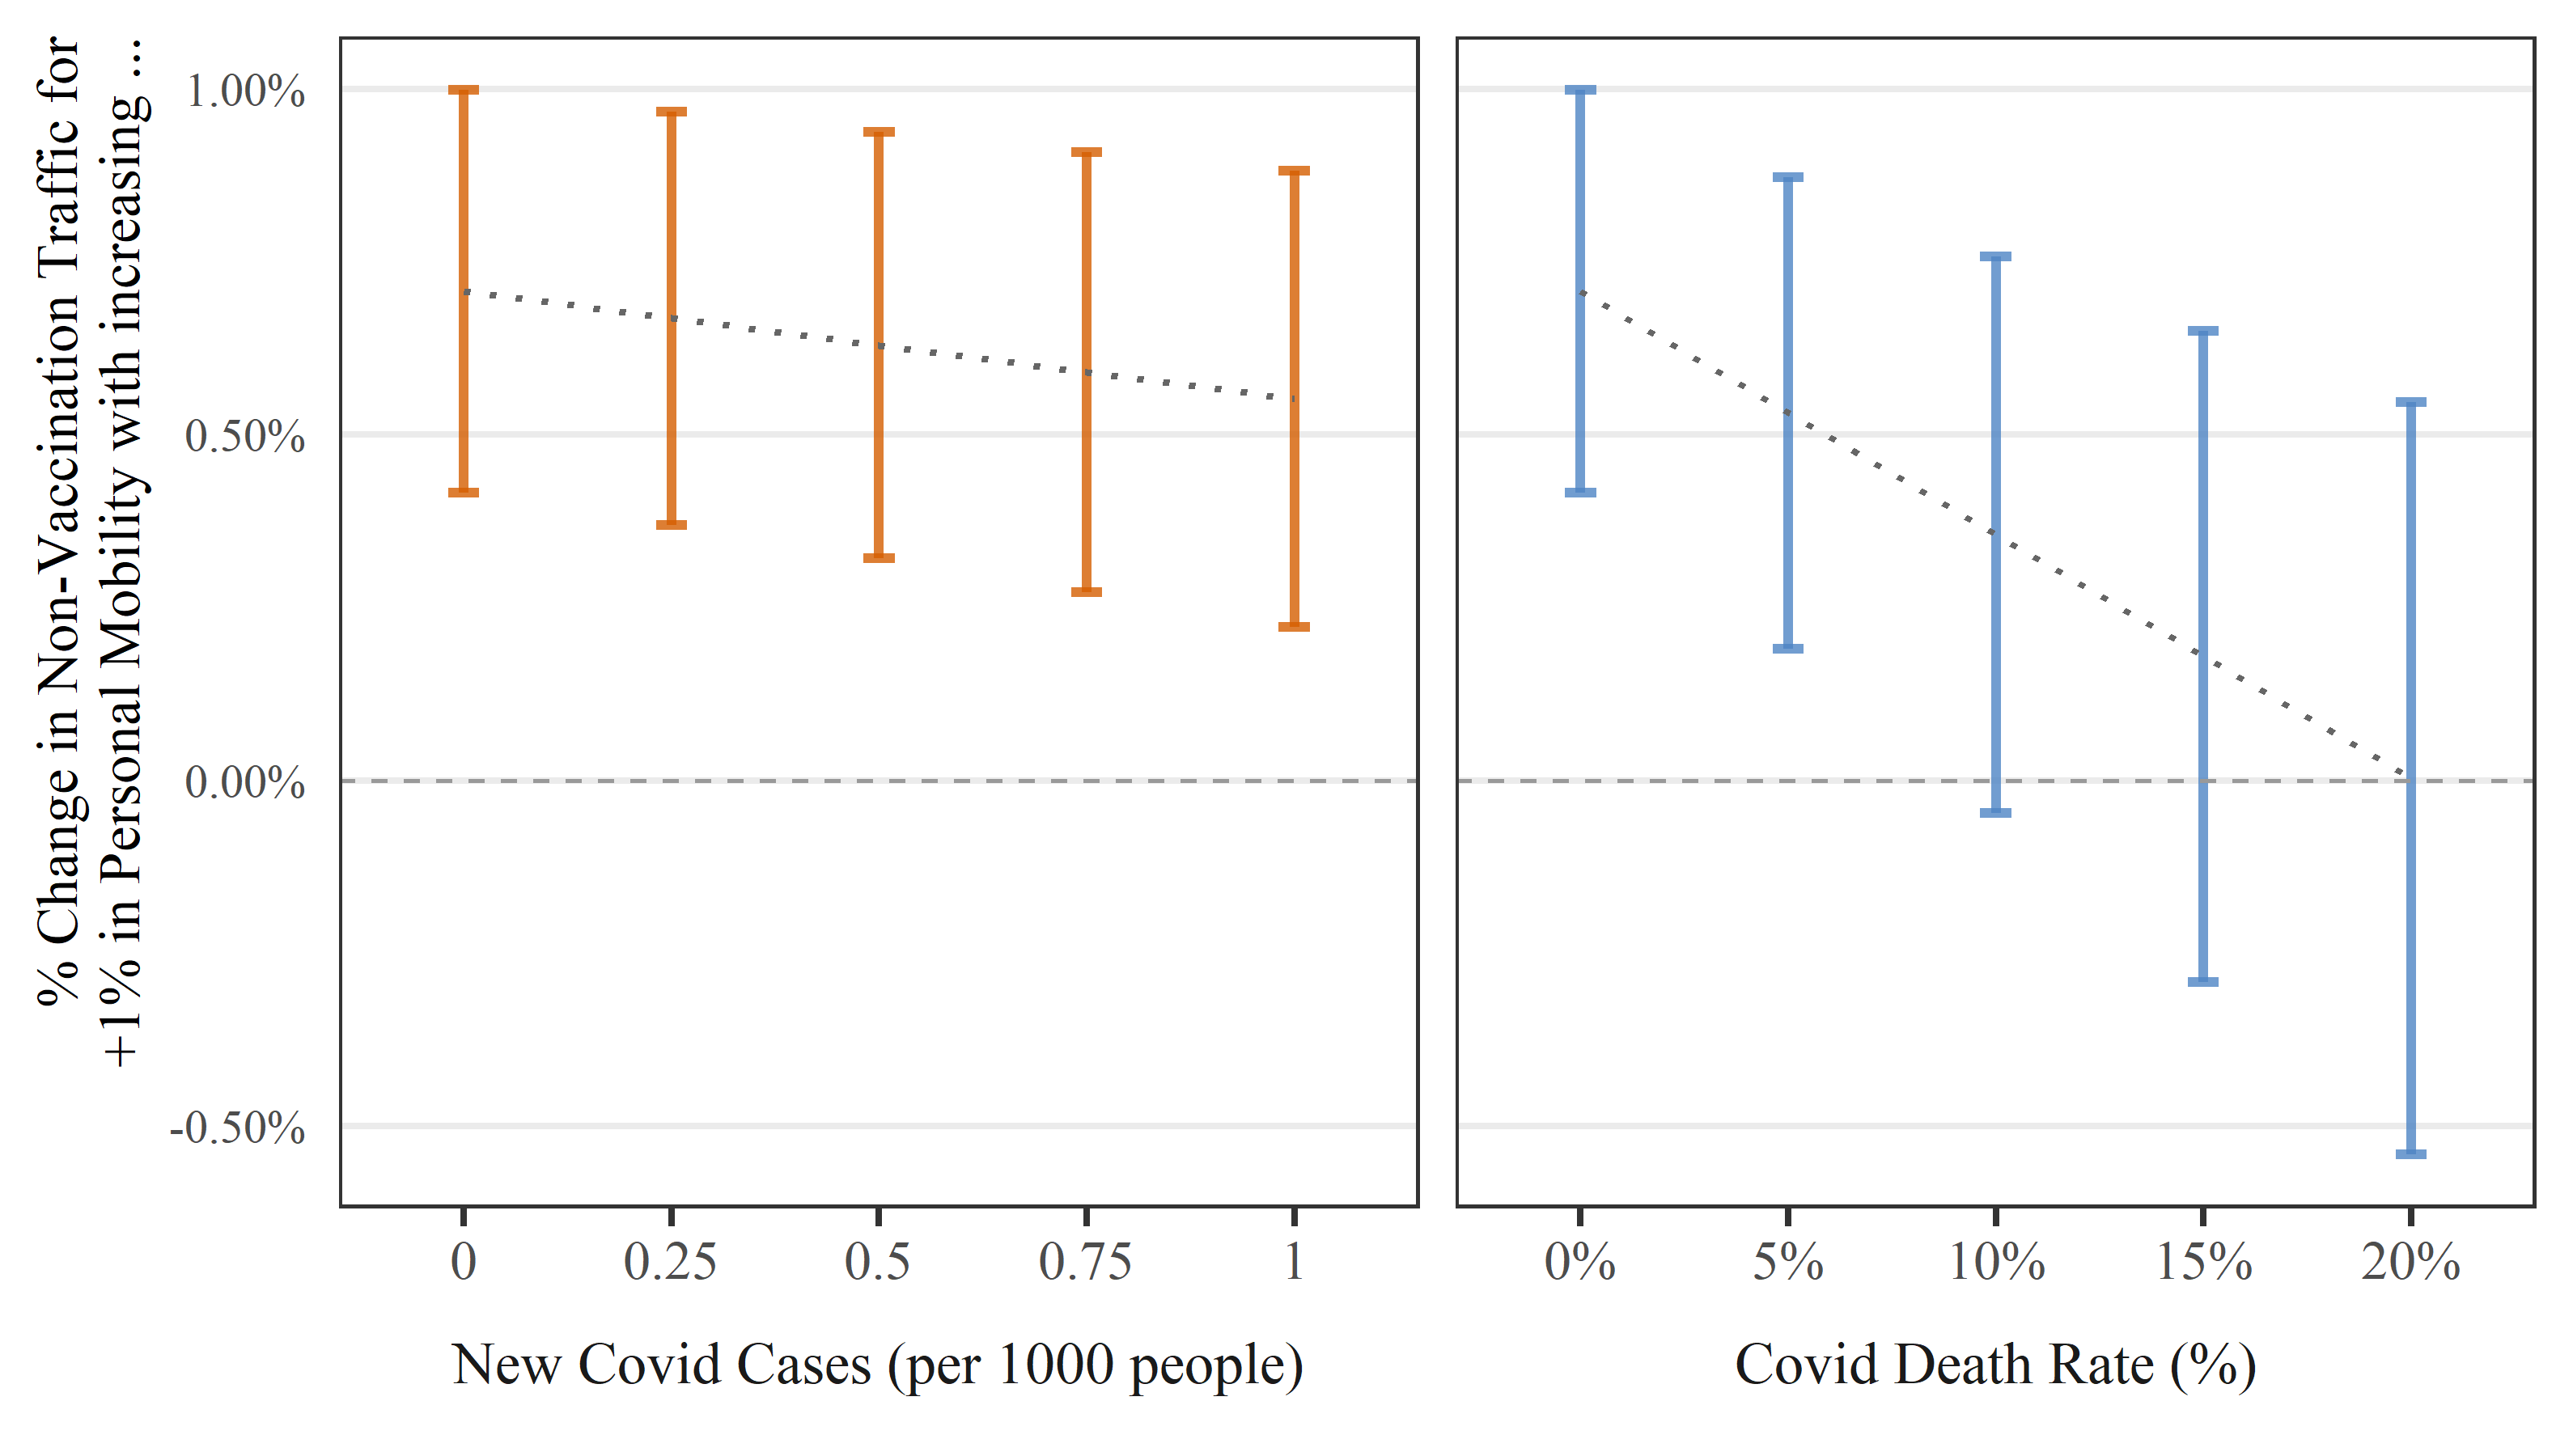
\includegraphics[scale=1]{Figures/VC2/Traffic-Moderation.png}     
    \label{fig:tfk_mod}
    % \floatfoot{\textbf{Figure Note:} 95\% confidence intervals depicted.}
\end{figure} 


\section{Conclusion} \label{VC2_Conc}
 Though recent technological innovations may have altered healthcare visits for good \citep{WSJ_checkup}, many aspects of medicine cannot happen virtually. Understanding the drivers of clinic traffic remains paramount, especially since a record number of patients delayed some type of care during the Covid-19 pandemic \citep{Findling2020}, where serious consequences can follow delayed or omitted vaccinations \citep{Salmon2015}. On top of this, the underlying causes of such concerns show few signs of abating as the emergence of Covid-19 variants continues to inhibit recovery \citep{WSJ_delta}.
 
 Combining observations from multiple sources allows us to evaluate how visits to healthcare clinics change with individual willingness to travel and signals of the current environment. As depicted in Figure \ref{fig:coef_plot}, increases in willingness to travel consistently drive large returns to vaccination traffic and smaller returns to all other traffic. Though the decreases in general clinic traffic do present some concerns, vaccination traffic seems immune to factors which depress demand for other care, such as such as state-wide stay-at-home orders and signals which might indicate a hazardous environment (e.g., a high Covid death rate). 
 
 We note the following limitations of our study. First, since observations of clinic traffic come from a vaccine management company, we observe only labels for “vaccination" or “non-vaccination" traffic. That is, we cannot identify different types of non-vaccination visits, even though some visits likely yield more value. Second, our data does not specify whether a non-vaccination visit happened virtually or in-person. Even so, Figure \ref{fig:model_free_vc2} shows non-vaccination traffic (virtual or otherwise) still had not recovered by the end of our study period. Said differently: Even with the broader acceptance and greater availability of telemedicine during the pandemic, such visits still cannot compensate for the drops we see in non-vaccination traffic. Third, we cannot observe the origin of a patient trip, though we do not believe patients cross multiple county lines to seek out primary care during the pandemic. Finally, we do not observe changes to clinic capacity in the wake of the pandemic. But since vaccination traffic returned to pre-pandemic baselines, we do not believe capacity restrictions hinder the recovery of non-vaccination traffic.
 
 Our findings yield several \textbf{implications} for research and practice. First, since mobility preferences strongly predict clinic traffic, operations managers can anticipate changes in traffic with greater precision by including such preferences in traffic prediction algorithms. Per one VaxCare representative: “Forecasting demand for vaccinations has been really tough recently. It is unclear what variables, if any, might be surrogates [for demand] which would reliably strengthen our forecasts." Our results show that personal mobility could be one such predictor.
 
 Second, clinicians can find solace knowing that even if mobility (and thus traffic) declines again, patient discretion can help weather steep drops. The public health community championed the benefits of vaccines for decades \citep{Brewer2017}, and the efforts paid off during the summer of 2020. To hedge future downturns, clinicians should continue broadcasting the value of important services.
 
 Third, policy makers should remember traffic flows from mobility. To restore patient traffic and minimize delayed care -- by all means, keep clinics open -- but also address the circumstances depressing mobility. Aside from critically important traffic, people will stay home until it feels safe. On the flip side: To discourage mobility and keep people at home, transmit at least some precise information. For example, if public health agencies had transmitted precise, severe signals (e.g., the Covid death rate) along with the stay-at-home orders, compliance with stay-at-home orders might have been less of an issue. 
 
 Finally, healthcare researchers must acknowledge the role patient discretion plays in affecting operational outcomes. During the pandemic, clinics remained open while patients exercised discretion in ways many feared \citep{WSJ_famVacc}. But instead of the forecasted apocalypse, we find patients prioritized important services and shouldered some of the burden in maintaining their own wellness. Going forward, researchers should suggest ways firms can leverage the patient in the co-production of health.
 
 Covid-19 threatened the lives of many patients; weakened traffic threatened the jobs of many clinicians. But in healthcare, both pursue a joint goal. We show that by working together, even in the midst of a pandemic, patients and clinics can achieve such a goal: A healthy patient living in a healthy environment.

 \begin{figure}
    \centering
    \caption{An increase in personal mobility consistently corresponds to a much stronger return to vaccination traffic than to non-vaccination traffic.} %\medskip
    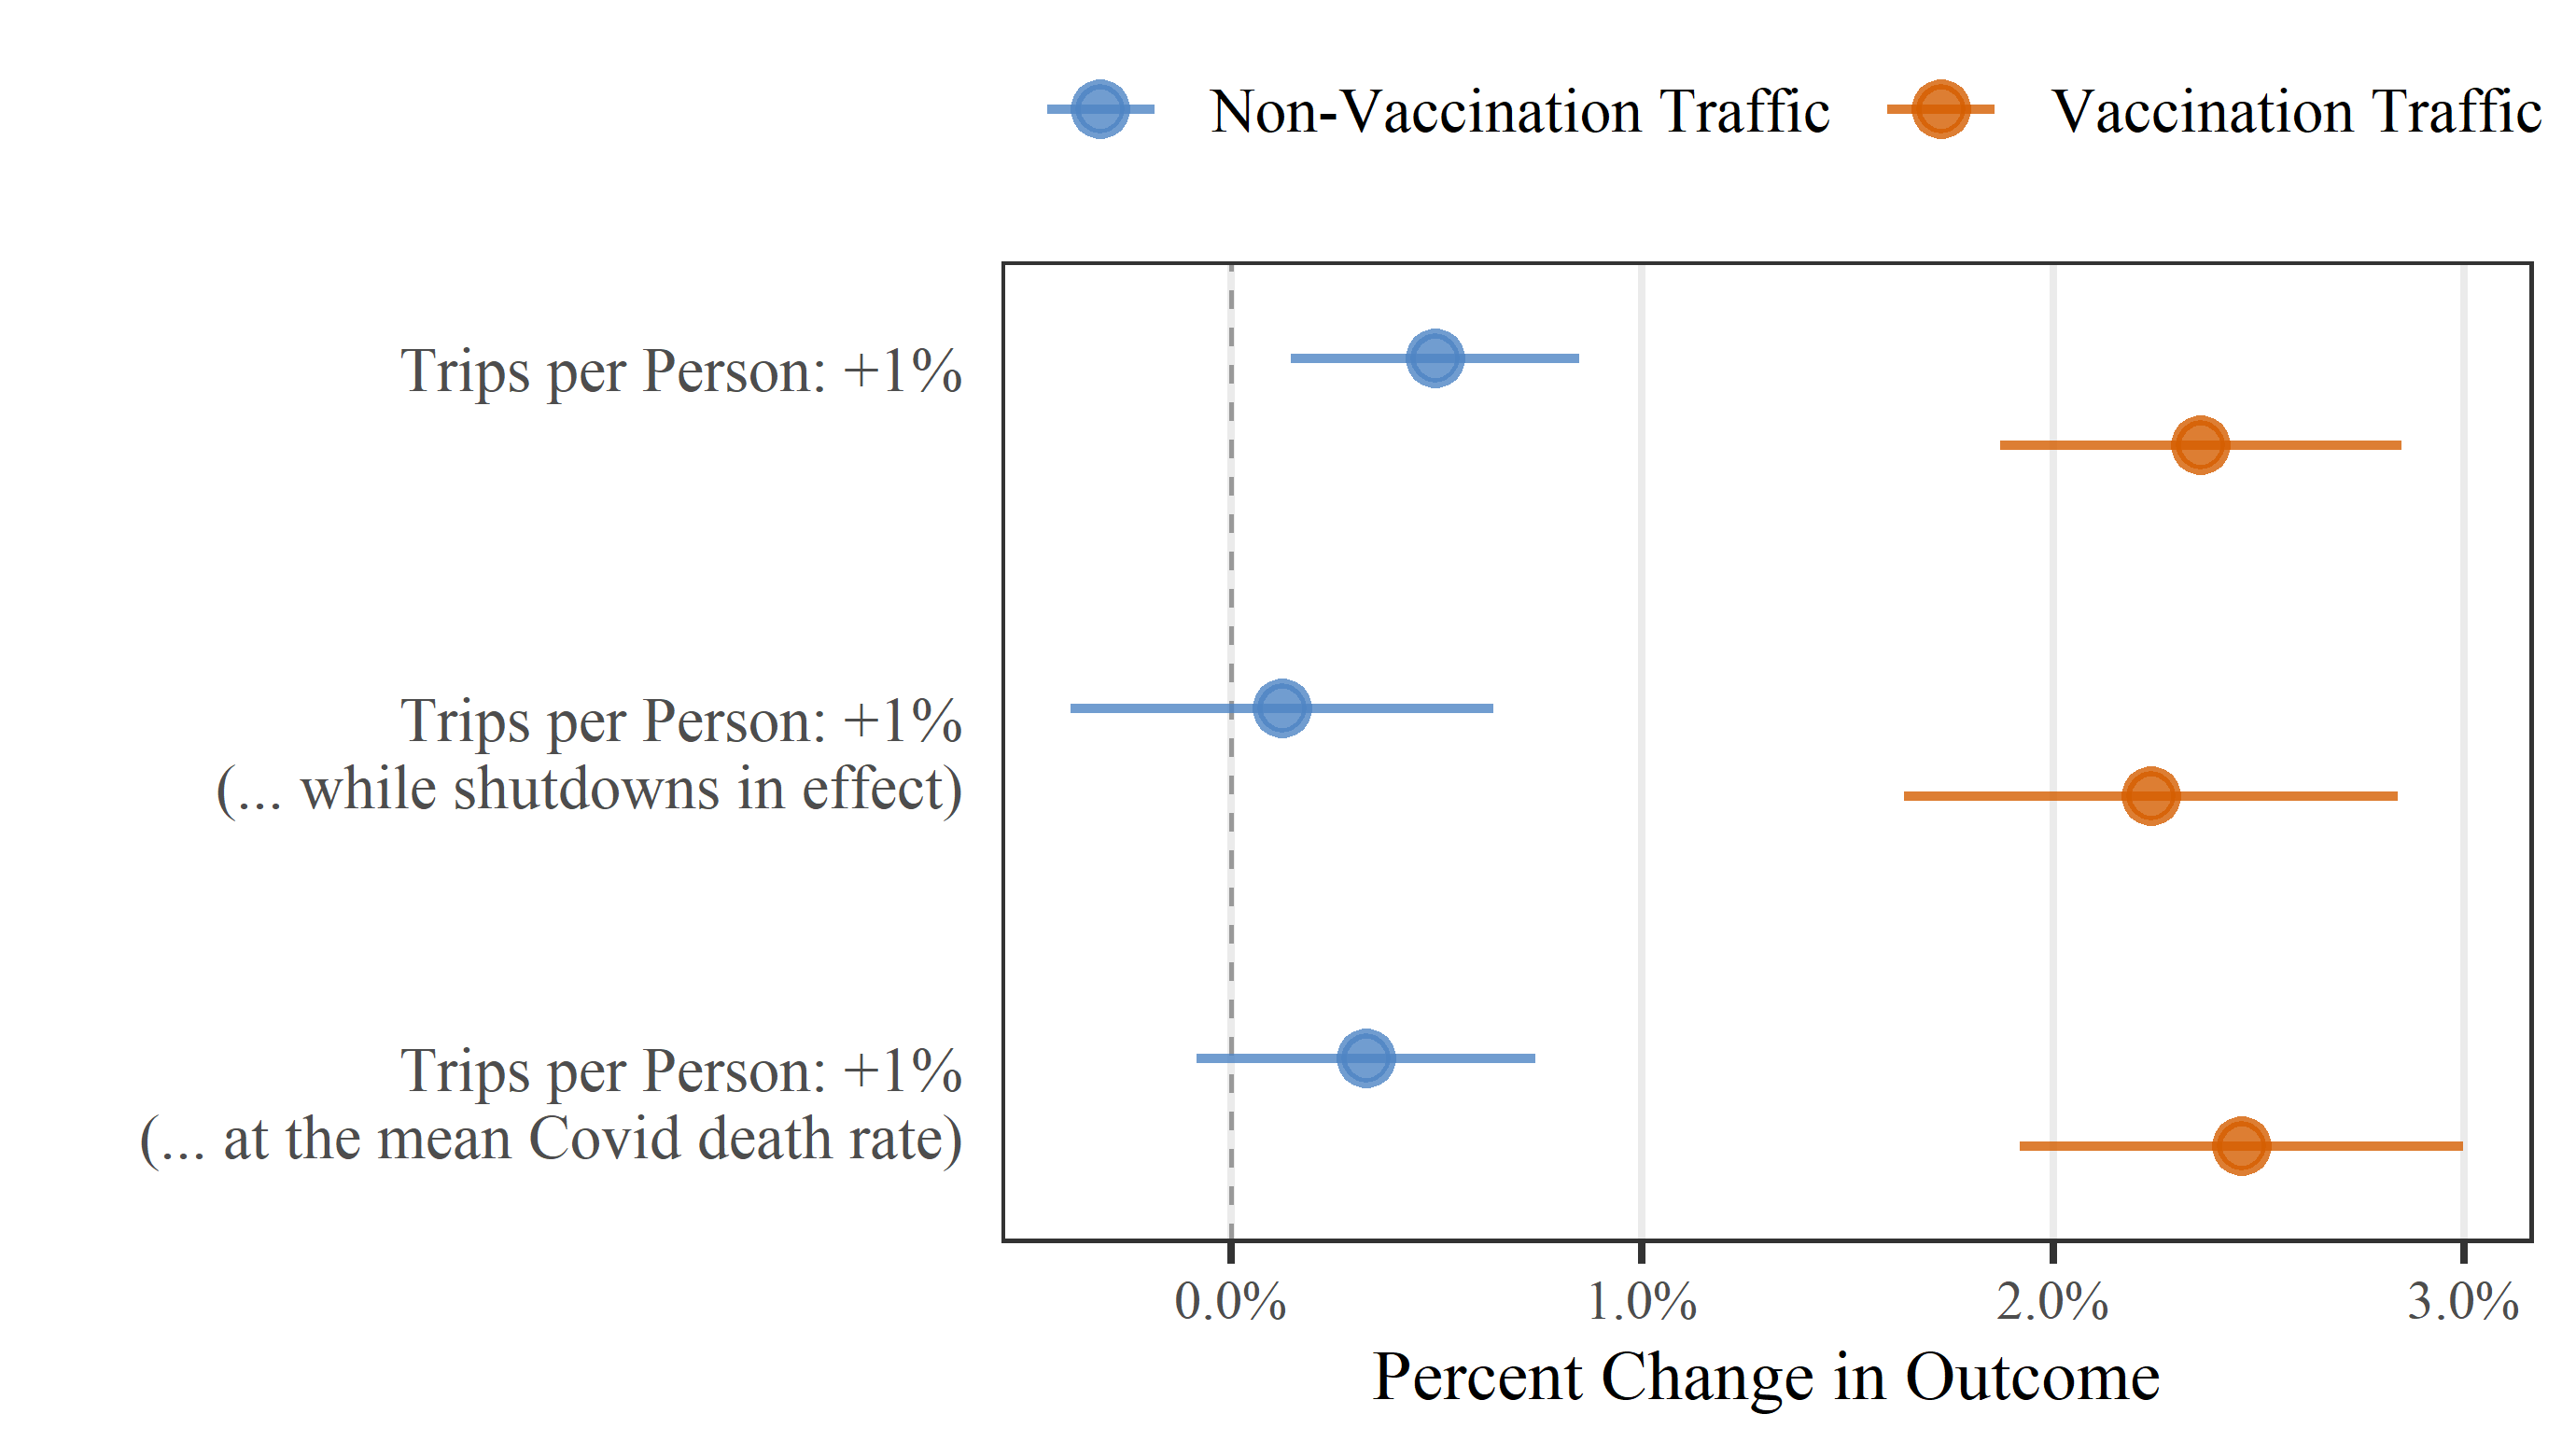
\includegraphics[scale=1]{Figures/VC2/Coef-Plot.png}     
    \label{fig:coef_plot}
    \floatfoot{\textbf{Figure Note:} The coefficient plot illustrates the marginal effect, or elasticity (and 95\% confidence intervals), of a change in personal mobility (i.e., Trips per Person) on clinic non-vaccination clinic traffic and vaccination traffic, as reported by the coefficients of Tables \ref{tab:H1H2} and \ref{tab:phoc}. The \nth{1} row illustrates a 1\% increase in personal mobility yields a more than 2\% increase in vaccination traffic versus a 0.5\% increase in non-vaccination traffic. The \nth{2} row depicts a significant drop in the effect of mobility on non-vaccination traffic while the state-wide stay-at-home orders are in effect, without a corresponding drop for vaccination traffic (Table \ref{tab:H1H2}, Columns 4 and 5). And the \nth{3} row illustrates that while the Covid death rate attenuates the effect of mobility on non-vaccination traffic, the effect of mobility on vaccination traffic seems immune to a such an effect (Table \ref{tab:phoc}).}
 \end{figure}
 
 